% Diagram for the report (er). Build: see build.sh in this folder.
\documentclass[12pt]{standalone}
% Shared style of every diagram and chart in the report.
% Each agent keeps the same colour in every figure.
% The diagrams are drawn here, not in main.tex, so the report itself does not
% load TikZ: it includes the built PDFs and compiles within Overleaf's time limit.
\usepackage{amsmath,amssymb}
\usepackage{xcolor}
\usepackage{tikz}
\usetikzlibrary{positioning,arrows.meta,shapes.geometric,shapes.misc,fit,calc,backgrounds}
\usepackage{pgfplots}
\pgfplotsset{compat=1.18}

% Same text width as the report (A4, 30 mm + 20 mm margins), for the charts.
\setlength{\textwidth}{160mm}
\newcommand{\Rs}{Rs.\,}
\newcommand{\code}[1]{\texttt{\detokenize{#1}}}

\definecolor{ink}{HTML}{2B2B2B}
\definecolor{agAfill}{HTML}{E4F2E1}\definecolor{agAline}{HTML}{3E7D3A} % Agent 1 Document & Vendor
\definecolor{agBfill}{HTML}{FCEBD5}\definecolor{agBline}{HTML}{B8701D} % Agent 2 Approval & Inventory
\definecolor{agCfill}{HTML}{EEE4F4}\definecolor{agCline}{HTML}{6E4A8E} % Agent 3 Contract & Risk
\definecolor{agDfill}{HTML}{FBE4E4}\definecolor{agDline}{HTML}{A8474B} % Agent 4 Platform
\definecolor{infill}{HTML}{E8EDF6}\definecolor{inline}{HTML}{4F6188}    % infrastructure / data
\definecolor{exfill}{HTML}{F2F2F2}\definecolor{exline}{HTML}{6F6F6F}    % people and external systems
\definecolor{humfill}{HTML}{FFF6D6}\definecolor{humline}{HTML}{9A7B12}  % human decision points
\definecolor{chartA}{HTML}{9AA5B1}\definecolor{chartB}{HTML}{3F5E8C}    % chart: baseline / shipped

\tikzset{
  >={Stealth[length=2mm]},
  every picture/.style={font=\footnotesize, line width=0.6pt, draw=ink, text=ink},
  nohyph/.style={execute at begin node={\hyphenpenalty=10000\exhyphenpenalty=10000}},
  box/.style={nohyph, draw, rounded corners=2pt, align=center, inner sep=3pt, minimum height=8mm},
  agA/.style={box, fill=agAfill, draw=agAline},
  agB/.style={box, fill=agBfill, draw=agBline},
  agC/.style={box, fill=agCfill, draw=agCline},
  agD/.style={box, fill=agDfill, draw=agDline},
  infra/.style={box, fill=infill, draw=inline},
  ext/.style={box, fill=exfill, draw=exline},
  human/.style={box, fill=humfill, draw=humline},
  decision/.style={nohyph, diamond, aspect=2.2, draw=humline, fill=humfill, align=center, inner sep=1pt},
  flow/.style={->, draw=ink},
  dflow/.style={->, draw=ink, dashed},
  lbl/.style={font=\scriptsize\itshape, fill=white, inner sep=1pt},
  note/.style={font=\scriptsize\itshape, align=center},
}
\pgfplotsset{
  reportbars/.style={
    ybar, width=0.95\textwidth, height=6cm, ymin=0,
    enlarge x limits=0.18, bar width=11pt,
    ymajorgrids, grid style={draw=black!12},
    axis line style={draw=black!60}, tick style={draw=black!60},
    legend style={draw=none, font=\footnotesize, legend columns=-1, at={(0.5,1.03)}, anchor=south},
    tick label style={font=\footnotesize}, label style={font=\footnotesize},
    nodes near coords, every node near coord/.append style={font=\scriptsize},
    /tikz/every even column/.append style={column sep=0.6cm},
    legend image code/.code={\draw[#1, draw=none] (0cm,-0.1cm) rectangle (0.3cm,0.1cm);},
  },
}

\begin{document}
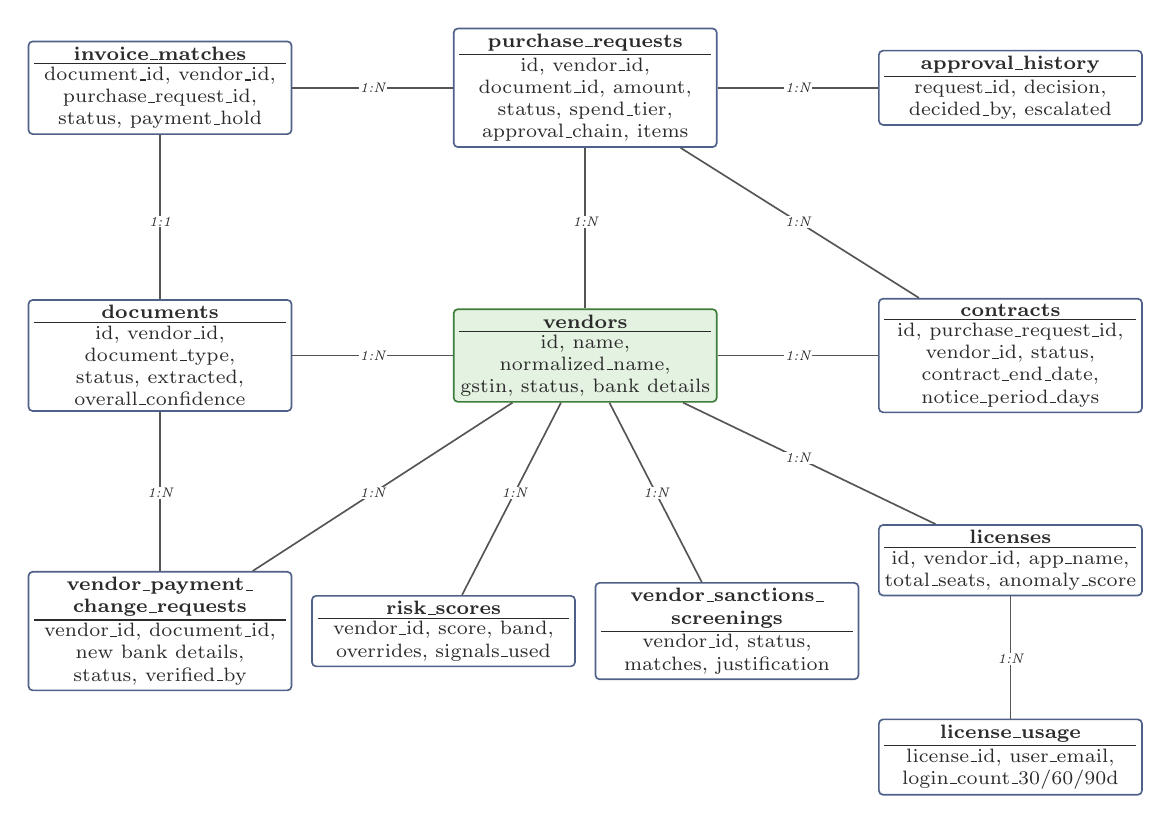
\begin{tikzpicture}
\tikzset{ent/.style={nohyph, draw=inline, fill=white, rounded corners=1.5pt, align=center, inner sep=2pt, text width=3.2cm, font=\scriptsize}, rel/.style={draw=ink!80}, card/.style={font=\tiny\itshape, fill=white, inner sep=0.5pt}}
\newcommand{\ent}[2]{\textbf{#1}\\[1pt]\hrule\vspace{1pt}#2}
\node[ent, fill=agAfill, draw=agAline] (v) at (0,0.9) {\ent{vendors}{id, name, normalized\_name, gstin, status, bank details}};
\node[ent] (pr) at (0,4.3) {\ent{purchase\_requests}{id, vendor\_id, document\_id, amount, status, spend\_tier, approval\_chain, items}};
\node[ent] (im) at (-5.4,4.3) {\ent{invoice\_matches}{document\_id, vendor\_id, purchase\_request\_id, status, payment\_hold}};
\node[ent] (ah) at (5.4,4.3) {\ent{approval\_history}{request\_id, decision, decided\_by, escalated}};
\node[ent] (d) at (-5.4,0.9) {\ent{documents}{id, vendor\_id, document\_type, status, extracted, overall\_confidence}};
\node[ent] (c) at (5.4,0.9) {\ent{contracts}{id, purchase\_request\_id, vendor\_id, status, contract\_end\_date, notice\_period\_days}};
\node[ent] (pc) at (-5.4,-2.6) {\ent{vendor\_payment\_\\change\_requests}{vendor\_id, document\_id, new bank details, status, verified\_by}};
\node[ent] (rs) at (-1.8,-2.6) {\ent{risk\_scores}{vendor\_id, score, band, overrides, signals\_used}};
\node[ent] (ss) at (1.8,-2.6) {\ent{vendor\_sanctions\_\\screenings}{vendor\_id, status, matches, justification}};
\node[ent] (l) at (5.4,-1.7) {\ent{licenses}{id, vendor\_id, app\_name, total\_seats, anomaly\_score}};
\node[ent] (lu) at (5.4,-4.2) {\ent{license\_usage}{license\_id, user\_email, login\_count\_30/60/90d}};
\foreach \a/\b/\c in {v/d/1:N, v/pr/1:N, v/c/1:N, v/pc/1:N, v/rs/1:N, v/ss/1:N, v/l/1:N, pr/ah/1:N, pr/c/1:N, l/lu/1:N, pr/im/1:N, d/im/1:1, d/pc/1:N}
  { \draw[rel] (\a) -- (\b); \node[card] at ($(\a)!0.5!(\b)$) {\c}; }
\end{tikzpicture}
\end{document}
